%iffalse
\let\negmedspace\undefined
\let\negthickspace\undefined
\documentclass[journal,12pt,twocolumn]{IEEEtran}
\usepackage{cite}
\usepackage{amsmath,amssymb,amsfonts,amsthm}
\usepackage{algorithmic}
\usepackage{graphicx}
\usepackage{textcomp}
\usepackage{xcolor}
\usepackage{txfonts}
\usepackage{listings}
\usepackage{enumitem}
\usepackage{mathtools}
\usepackage{gensymb}
\usepackage{comment}
\usepackage[breaklinks=true]{hyperref}
\usepackage{tkz-euclide} 
\usepackage{listings}
\usepackage{gvv}                                        
%\def\inputGnumericTable{}                                 
\usepackage[latin1]{inputenc}                                
\usepackage{color}                                            
\usepackage{array}                                            
\usepackage{longtable}                                       
\usepackage{calc}                                             
\usepackage{multirow}                                         
\usepackage{hhline}                                           
\usepackage{ifthen}                                           
\usepackage{lscape}
\usepackage{tabularx}
\usepackage{array}
\usepackage{float}


\newtheorem{theorem}{Theorem}[section]
\newtheorem{problem}{Problem}
\newtheorem{proposition}{Proposition}[section]
\newtheorem{lemma}{Lemma}[section]
\newtheorem{corollary}[theorem]{Corollary}
\newtheorem{example}{Example}[section]
\newtheorem{definition}[problem]{Definition}
\newcommand{\BEQA}{\begin{eqnarray}}
\newcommand{\EEQA}{\end{eqnarray}}
\newcommand{\define}{\stackrel{\triangle}{=}}
\theoremstyle{remark}
\newtheorem{rem}{Remark}
\begin{document}

\bibliographystyle{IEEEtran}
\vspace{3cm}

\title{11.9.3.17}
\author{EE23BTECH11017 - Eachempati Mihir Divyansh$^{*}$% <-this % stops a space
}
\maketitle
\newpage
\bigskip

\renewcommand{\thefigure}{\theenumi}
\renewcommand{\thetable}{\theenumi}

\textbf{Question: }
If the $4^{th}$, $10^{th}$ and $16^{th}$ terms of a G.P. are x, y, and z, respectively. Prove that $x,\; y,\; z$ are in G.P.


\begin{table}[h]
    \renewcommand\thetable{1}
    \centering
        \caption{\textbf{Given Information}}
        \begin{tabular}{|m{2cm}|m{2cm}|m{2cm}|}
    \hline
    \textbf{Symbol} & \textbf{Value} & \textbf{Description}\\ [1ex]
    \hline
        $x$ & $x\brak{0}r^3$ & $x\brak{3}$ \\ [1ex]
    \hline
        $y$ & $x\brak{0}r^{9}$ & $x\brak{9}$\\ [1ex]
    \hline
        $z$ & $x\brak{0}r^{15}$ & $x\brak{15}$\\ [1ex]
    \hline
        $r$ & $y^{\frac{1}{6}}x^{-\frac{1}{6}}$ & $\frac{x\brak{n}}{x\brak{n-1}}$\\[1ex]
    \hline \vspace{0.1cm}
        $x\brak{0}$ & $x^{\frac{3}{2}}y^{-\frac{1}{2}}$ & First term \\[1ex]
    \hline
        $x\brak{n}$ & $x\brak{0}r^nu\brak{n}$ & General Term \\ [1ex]
    \hline
    \end{tabular}
\label{Table 1}
\end{table} 

\solution

\begin{enumerate}
\item From \tabref{Table 1},
\begin{align}
    x&= x\brak{4} =x\brak{0}r^4 \\
 y&=x\brak{10}=x\brak{0}r^{10} \\
 z&=x\brak{16}=x\brak{0}r^{16}
\end{align}
Consider $\dfrac{x\brak{10}}{x\brak{4}}$ and $\dfrac{x\brak{16}}{x\brak{10}}$;
\begin{align}
 \implies\dfrac{x\brak{10}}{x\brak{4}} &= \dfrac{x\brak{0}r^{10}}{x\brak{0}r^4} = r^6 \label{Eqn 4}\\ 
 \implies\dfrac{x\brak{16}}{x\brak{10}} &= \dfrac{x\brak{0}r^{16}}{x\brak{0}r^{10}} = r^6\label{Eqn 5}
\end{align}
From \eqref{Eqn 4} and \eqref{Eqn 5}
\begin{align}  
   & x\brak{4},\; x\brak{10},\; x\brak{16}\text{ are in G.P.} \\
\notag  \therefore & x,\; y,\; z \text{ are in G.P.}
\end{align}
\item
$x\brak{0}$ and $r$ can be expressed in terms of $x$, $y$, and $z$ in the following manner.
\begin{align}
    \implies&\frac{y}{x}=r^6 \\
 \implies& r=\sqrt[6]{\frac{y}{x}}=\brak{\frac{y}{x}}^{\frac{1}{6}}\\
    \implies&  x=x\brak{0}r^4 \\
    \implies& x\brak{0}=\frac{x}{r^4}\\
    &=x\brak{\frac{x}{y}}^{\frac{4}{6}}\\
 \therefore\; x\brak{0}&=x^{\frac{5}{3}}y^{-\frac{2}{3}}\;
 \text{and}\; r=\brak{\frac{y}{x}}^{\frac{1}{6}}= y^{\frac{1}{6}}x^{-\frac{1}{6}} \label{Eqn 13}
\end{align}
\item 
Z-transform:    $x\brak{n} \system{Z} X\brak{z}$
\begin{align}
    X\brak{z}&= \sum_{n=-\infty}^{\infty} x\brak{n}z^{-n}\\
    X\brak{z}&=\dfrac{x\brak{0}}{1-rz^{-1}}\: \forall\: |z|>|r|
\end{align}
Substituting $r$ and $x\brak{0}$ from \eqref{Eqn 13}, 
\begin{align}
     X\brak{z}&=\dfrac{x^{\frac{5}{3}}y^{-\frac{2}{3}}}{1-{\brak{\frac{y}{x}}^{\frac{1}{6}}}z^{-1}}
\end{align}
\item Example 
\begin{align}
    \notag\text{Let}\;x\brak{0} =\dfrac{1}{256}\;\text{and}\;r = 2\\     \notag x=x\brak{4}=x\brak{0}r^4 &=\frac{1}{256}\brak{2}^4=\frac{1}{16}\\
     \implies x&=\frac{1}{16} \\
    \notag y=x\brak{10}=x\brak{0}r^{10} &=\frac{1}{256}\brak{2}^{10}=4\\
     \implies y&=4 \\
    \notag z=x\brak{16}=x\brak{0}r^{16} &=\frac{1}{256}\brak{2}^{16}=256\\
    \implies z&=256 
\end{align}
\newpage
\begin{figure}[h]
    \renewcommand\thefigure{1}
    \centering
    \caption{Stem Plot of $x(n)$ v/s $n$}
   % \caption{Stem Plot of $x(n)$ vs $n$}
    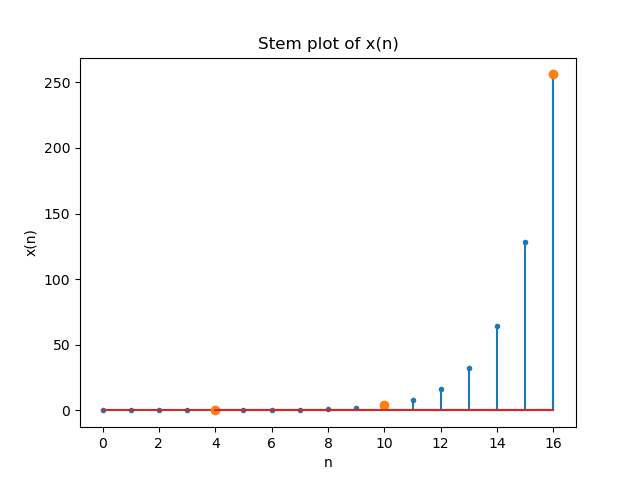
\includegraphics[width=\columnwidth]{A_1.png}
        \label{fig:1}
\end{figure}


\end{enumerate}

\end{document}
